\input kzllyyhead

%%%%%%%%%%%%%%%%%%%%%%%%%%%%%%%%%%%%%%%%%%%%%%%%%%%%%%%%%%%%%%%%
%      文章正文
%%%%%%%%%%%%%%%%%%%%%%%%%%%%%%%%%%%%%%%%%%%%%%%%%%%%%%%%%%%%%%%%
\begin{document}
%%%%%%%%%%%%%%%%%%%%%%%%%%%%%%%%%%%%%%%%%%%%%%%%%%%%%%%%%%%%%%%%
% 标题，基金项目，作者，地址定义
%%%%%%%%%%%%%%%%%%%%%%%%%%%%%%%%%%%%%%%%%%%%%%%%%%%%%%%%%%%%%%%%
\makeatother
\title{\LARGE\textbf{基于多输入多输出状态空间模型的人形机器人轻量级世界模型}\\
\footnotetext{\scriptsize \hskip -6pt
\hspace*{-0.1em}收稿日期: xxxx$-$xx$-$xx; 录用日期: xxxx$-$xx$-$xx.\\
\hspace*{1.1em}$^{\dag}$通讯作者. E-mail: \mbox{semhaqx@gmail.com}.\\
\hspace*{1.1em}本文责任编委: XXX.\\
\hspace*{1.1em}国家社会科学基金项目(21BGL231), 湘江实验室重大项目(24XJ01001; 25XJ01001)资助.\\
\hspace*{1.1em}Supported by the National Social Science Fund of China (21BGL231) and the
Major Program of Xiangjiang Laboratory (24XJ01001; 25XJ01001).}}
\author{{\large {\CJKfamily{fsong}周新民\makebox{$^{1,\,2}$},~~余焕杰\makebox{$^{3}$}\makebox{$^{\dag}$},~~张慧慧\makebox{$^{4}$},~~王伟\makebox{$^{3}$},~~陈露\makebox{$^{4}$}}}\\
\scriptsize
(1. 湖南工商大学~人工智能与机器人学院, 湖南~长沙~410205;\\
\scriptsize 2. 湘江实验室, 湖南~长沙~410205;\\
\scriptsize 3. 湖南工商大学~计算机学院, 湖南~长沙~410205;\\
\scriptsize 4. 湖南工商大学~前沿交叉学院, 湖南~长沙~410205) \\}
\date{}
\fancyhead[CO]{{\footnotesize 周新民等: 基于多输入多输出状态空间模型的人形机器人轻量级世界模型}}
\setlength{\abovedisplayskip}{1.5mm}
\setlength{\belowdisplayskip}{1.5mm}
\maketitle
%%%%%%%%%%%%%%%%%%%%%%%%%%%%%%%%%%%%%%%%%%%%%%%%%%%%%%%%%%%%%%%%
%      中文摘要
%%%%%%%%%%%%%%%%%%%%%%%%%%%%%%%%%%%%%%%%%%%%%%%%%%%%%%%%%%%%%%%%
\setlength{\oddsidemargin}{ 1cm}
\setlength{\textwidth}{15.5cm} \vspace{-1.2cm}
\begin{center}
\parbox{\textwidth}{\setlength{\parindent}{1em}
{\footnotesize {\CJKfamily{hei} 摘要:}
针对人形机器人高维状态预测中精度与计算效率难以兼顾的问题, 本文提出一种基于多输入多输出状态空间模型的轻量级世界模型MIMO-WM.
该模型通过并行扫描算法实现高效序列建模, 并引入sigmoid门控机制增强表达能力.
在Gymnasium MuJoCo基准的Humanoid和HumanoidStandup两个人形机器人数据集上的多种子实验表明, MIMO-WM在Humanoid上取得最优精度, 均方误差为$19.87\times10^{-2}$, 比次优方法降低1.5\%, 参数量仅0.138M.
理论分析证明了对角状态空间模型递推与卷积模式的等价性、计算复杂度优势以及交叉熵方法采样式模型预测控制的收敛性.
实验结果验证了MIMO-WM在人形机器人状态预测任务中的有效性和轻量化优势.

{\CJKfamily{hei} 关键词:} 状态空间模型; 世界模型; 状态预测; 模型预测控制; 具身智能

{\CJKfamily{hei}引用格式:} 周新民, 余焕杰, 张慧慧, 等. 基于多输入多输出状态空间模型的人形机器人轻量级世界模型. 控制理论与应用, xxxx, xx(x): xxx -- xxx\\\vspace*{-16pt}

\textbf{DOI:} 10.7641/CTA.202x.xxxxx

\textbf{代码开源:} \texttt{https://github.com/SEMHAQ/MIMO-WM}
}}
\end{center}
%%%%%%%%%%%%%%%%%%%%%%%%%%%%%%%%%%%%%%%%%%%%%%%%%%%%%%%%%%%%%%%%
%          英文摘要
%%%%%%%%%%%%%%%%%%%%%%%%%%%%%%%%%%%%%%%%%%%%%%%%%%%%%%%%%%%%%%%%
\vspace{.1cm}
\begin{center}
\parbox{\textwidth}{\setlength{\parindent}{1em}
{\centering\large\textbf{A Lightweight MIMO-SSM World Model for Humanoid Robot State Prediction}} \vspace{-1.2mm}
\begingroup\centering
ZHOU Xin-min$^{1,\,2}$,~~YU Huan-jie$^{3\dagger}$,~~ZHANG Hui-hui$^{4}$,~~WANG Wei$^{3}$,~~CHEN Lu$^{4}$\\[2pt]
\scriptsize{(1. School of Artificial Intelligence and Robotics, Hunan University of Technology and Business, Changsha Hunan 410205, China;\\
2. Xiangjiang Laboratory, Changsha Hunan 410205, China;\\
3. School of Computer Science, Hunan University of Technology and Business, Changsha Hunan 410205, China;\\
4. School of Frontier Crossover Studies, Hunan University of Technology and Business, Changsha Hunan 410205, China)}
\end{center}

\vspace{-10pt}\footnotesize{\textbf{Abstract:}
Humanoid robot state prediction faces the dual challenges of accuracy and computational efficiency. This paper proposes MIMO-WM, a lightweight world model based on multi-input multi-output state space model architecture, which achieves efficient sequence modeling through parallel scanning and enhances expressiveness via a sigmoid gating mechanism. Multi-seed experiments on Gymnasium MuJoCo Humanoid and HumanoidStandup benchmarks demonstrate that MIMO-WM achieves the best prediction accuracy on Humanoid with mean squared error of $19.87\times10^{-2}$, outperforming the second-best method by 1.5 percent, while requiring only 0.138 million parameters. Theoretical analysis proves the equivalence of recurrent and convolution computation modes, the computational complexity advantage, and the convergence guarantee of cross-entropy method based model predictive control. Experimental results validate the effectiveness and lightweight advantage of MIMO-WM for humanoid robot state prediction tasks.

\textbf{Key words:} state space model; world model; state prediction; model predictive control; embodied intelligence

\textbf{Citation:} X. Zhou, H. Yu, H. Zhang, et al. A lightweight MIMO-SSM world model for humanoid robot state prediction. {\it Control Theory \& Applications}, xxxx, xx(x): xxx -- xxx}}
\end{center}

\renewcommand\refname{\normalsize{{\CJKfamily{hei}参考文献}}}
%%%%%%%%%%%%%%%%%%%%%%%%%%%%%%%%%%%%%%%%%%%%%%%%%%%%%%%%%%%%%%%%
%  正文
%%%%%%%%%%%%%%%%%%%%%%%%%%%%%%%%%%%%%%%%%%%%%%%%%%%%%%%%%%%%%%%%
\setlength{\oddsidemargin}{-.5cm}
 \setlength{\textwidth}{171mm}
\CJKfamily{song}
\vspace{10pt}
\enlargethispage{-10mm}
\begin{multicols}{2}
\fontsize{10.5bp}{12.9bp}\selectfont

\section{引言}

具身智能的核心在于智能体通过与物理环境的实时交互来学习、进化并执行任务\textsuperscript{\cite{1}}.
机器人作为具身智能的重要载体, 其高维度、强非线性及欠驱动特性使得``感知--决策--控制"的闭环实现极具挑战.
其中, 世界模型\textsuperscript{\cite{2}}作为环境动力学的内部表征, 其核心功能包括:
(1)给定当前状态和动作预测未来状态(状态转移建模),
(2)预测奖励信号和终止条件,
(3)基于预测能力支持规划与决策.
在模型预测控制（model predictive control, MPC）框架中,
世界模型通过前向模拟多步未来状态轨迹为优化求解提供动力学约束,
其预测精度和推理速度直接决定了控制性能.

近年来, 基于深度学习的世界模型取得了显著进展.
基于循环神经网络（recurrent neural network, RNN）的方法\textsuperscript{\cite{3}}虽然能够建模时序依赖, 但存在梯度消失和长程依赖捕捉困难的问题.
基于Transformer的方法\textsuperscript{\cite{4}}通过自注意力机制有效解决了长程依赖问题,
但其二次计算复杂度$O(T^2)$在长序列场景下带来显著的计算开销.
在具身智能领域, RT-2\textsuperscript{\cite{5}}等大规模视觉-语言-动作模型展示了世界模型在机器人控制中的巨大潜力,
但其庞大的参数量和计算需求使得部署在资源受限的机器人平台上面临严峻挑战.

状态空间模型（state space model, SSM）\textsuperscript{\cite{6}}作为一种新兴的序列建模方法,
通过线性递推结构实现了$O(T)$的每步推理复杂度, 在长序列处理上具有天然优势.
从S4的结构化参数化到S4D\textsuperscript{\cite{7}}的对角简化,
再到Mamba\textsuperscript{\cite{8}}的选择性扫描机制, SSM在语言建模等任务上已取得与Transformer相当的性能\textsuperscript{\cite{9}}.

然而, 将SSM应用于具身智能领域的世界模型构建尚处于起步阶段.
现有工作主要集中在视觉感知和语言理解领域,
而在机器人状态预测和控制方面的探索相对有限.
近期, Mamba策略网络\textsuperscript{\cite{20,21}}和SSM时序预测\textsuperscript{\cite{22}}等工作开始将SSM引入机器人和序列决策领域,
但前者侧重于策略学习, 后者侧重于时序数据预测,
均未涉及面向机器人状态预测的世界模型构建.
机器人状态预测任务面临三重挑战: 状态维度高, 涉及多个关节的耦合动力学; 动作-状态映射具有强非线性; 且控制回路要求毫秒级的推理延迟.
这些特点要求世界模型在保持高预测精度的同时, 具备极低的计算开销.

更重要的是, 现有SSM方法在应用于机器人状态预测时存在根本性局限:
S4D}采用固定对角状态矩阵, 无法根据输入内容调整动力学特性,
而机器人系统的动力学参数如摩擦系数、惯性矩会随关节配置和运动状态变化;
Mamba}的选择性扫描机制虽然具有输入自适应能力, 但其参数量和计算开销较大,
不适合资源受限的机器人部署场景.
因此, 设计一种既能保持对角SSM的计算效率、又能适应机器人动力学变化的新型SSM架构, 是一个亟待解决的关键问题.

本文的主要贡献如下:

1)~~提出多输入多输出世界模型（Multi-Input Multi-Output World Model, MIMO-WM）, 通过对角SSM与sigmoid门控机制的结合, 在保持线性计算复杂度的同时实现更强的表达能力. 门控机制使模型能够根据输入内容动态调节信息流动, 参数量仅0.138M;

2)~~在Gymnasium MuJoCo基准的Humanoid和HumanoidStandup两个人形机器人数据集上进行了多种子实验. 结果表明MIMO-WM在Humanoid上取得最优精度, 均方误差为$19.87\times10^{-2}$, 比Mamba-WM降低1.5\%, 比Transformer-WM降低29.3\%, 同时参数量最少;

3)~~在机器人世界模型状态预测任务上系统比较了长短期记忆网络（long short-term memory, LSTM）、门控循环单元（gated recurrent unit, GRU）、Transformer、Mamba、时间卷积网络（temporal convolutional network, TCN）和MIMO-WM六种序列模型, 揭示了门控机制对SSM表达能力的显著提升;

4)~~理论分析证明了对角SSM递推与卷积模式的等价性、计算复杂度优势和交叉熵方法采样式MPC收敛性保证.

本文其余部分组织如下: 第2节回顾相关工作; 第3节介绍问题描述与预备知识; 第4节详述所提方法; 第5节给出实验结果与分析; 第6节总结全文并展望未来工作.

\section{相关工作}

\subsection{机器人世界模型}

世界模型的概念最早可追溯到Karl Friston的主动推理理论,
其核心思想是智能体通过构建环境的内部模型来进行预测和规划.
在深度学习时代, Ha和Schmidhuber提出了基于变分自编码器VAE和循环神经网络的世界模型框架,
通过学习压缩的环境表征来实现策略学习.
Hafner等人\textsuperscript{\cite{10}}提出了Dreamer系列方法, 利用潜在动力学模型在想象中进行策略优化,
在多个连续控制基准上取得了领先性能.
DreamerV3\textsuperscript{\cite{11}}进一步统一了离散和连续动作空间的处理, 展示了世界模型的通用性.

在机器人领域, Michels等人探索了利用世界模型进行视觉伺服控制.
Nagabandi等人\textsuperscript{\cite{12,13,14}}将神经网络动力学模型与模型预测控制相结合, 实现了机器人腿部运动的快速适应.
近期, RT-2}\textsuperscript{\cite{5}}将大规模视觉-语言模型与机器人动作空间对齐,
展示了基础模型在机器人控制中的潜力.
然而, 这些方法普遍面临计算开销大、难以满足实时控制要求的问题.
在高效计算方面, TinyML\textsuperscript{\cite{15}}和模型压缩技术为资源受限平台上的深度学习部署提供了解决方案.
在仿真到真实迁移方面, 域随机化和快速电机适应RMA等方法缩小了仿真与真实机器人之间的差距.
世界模型在自动驾驶领域也得到了广泛关注\textsuperscript{\cite{16}}, 连续-离散状态空间模型为混合系统建模提供了新思路.
本文提出的MIMO-WM旨在以极低的计算开销实现高质量的状态预测,
为机器人状态预测提供一种轻量级SSM-Attention混合解决方案.

\subsection{状态空间模型}

SSM源于控制理论中的线性系统描述,
近年来在深度学习领域引起了广泛关注.
Gu等人\textsuperscript{\cite{17}}提出的HiPPO框架通过最优多项式投影解决了连续时间记忆问题,
为SSM在序列建模中的应用奠定了理论基础.
S4}\textsuperscript{\cite{6}}通过结构化参数化
解决了SSM在长程依赖建模中的数值稳定性问题,
在Long Range Arena基准上取得了突破性结果.

在S4的基础上, 研究者提出了多种改进方案.
S4D简化了对角SSM的参数化, 直接使用复数对角矩阵,
在保持性能的同时显著降低了实现复杂度.
并行扫描算法\textsuperscript{\cite{18}}也被用于加速SSM的训练过程.
H3\textsuperscript{\cite{19}}结合了SSM与门控注意力, 在语言建模中取得了与Transformer相当的性能.

Mamba是SSM发展的一个重要里程碑.
它引入了选择性扫描机制, 使SSM的状态更新能够根据输入内容动态调整,
从而在保持线性计算复杂度的同时实现了与Transformer相当的建模能力.
Mamba的块结构已成为现代SSM架构的标准设计模式.
Mamba-2}\textsuperscript{\cite{9}}进一步揭示了SSM与注意力机制之间的结构化状态空间对偶性,
为统一理解不同序列建模方法提供了新的理论框架.

现有SSM方法在应用于机器人状态预测时存在局限性.
S4D采用固定对角参数化, 无法根据输入内容调整动力学特性;
Mamba的选择性扫描机制虽然具有输入自适应能力, 但其参数量和计算开销较大.
MIMO-SSM通过多输入多输出结构, 在保持对角SSM计算效率的同时实现了更强的表达能力,
参数量和计算开销远小于Mamba, 更适合资源受限的机器人部署场景.

近期SSM类方法开始在机器人领域得到应用.
在策略学习方面, Mamba被用于替代Transformer作为策略网络的主干}, 实现了更高效的序列决策,
其中Mamba策略网络}在连续控制任务中取得了与Transformer策略网络相当的性能,
但推理速度提升了2--3倍.
在时序预测方面, SSM被用于长程多变量时序预测}, 利用其线性复杂度和长程建模优势.
在世界模型方面, Dreamer系列}和TD-MPC}等方法主要基于循环神经网络或潜在动力学模型进行环境建模,
且主要面向视觉输入, 计算开销较大.
近期, RoboMamba\textsuperscript{\cite{23}}将Mamba与视觉编码器结合用于机器人操作,
但其侧重视觉-语言理解而非状态空间的动力学建模.

本文聚焦于状态-动作序列的世界模型构建, 区别于视觉输入的世界模型和策略网络方法,
MIMO-WM以极低的参数开销实现状态转移预测, 并通过MPC框架验证了其在规划决策中的可行性.

\subsection{轻量级模型与实时控制}

在资源受限的机器人平台上部署深度学习模型是一个重要挑战.
知识蒸馏、模型剪枝和量化是常用的模型压缩方法.
网络架构搜索（neural architecture search, NAS）也被用于自动设计高效的网络结构.
然而, 这些方法通常是事后压缩, 可能导致性能损失.

从架构设计角度出发, GRU通过简化LSTM的门控结构减少了参数量.
TCN利用因果卷积和膨胀卷积实现了高效的序列建模.
SSM类方法}通过线性递推结构实现了$O(T)$的每步推理复杂度和$O(1)$的单步延迟,
在长序列场景下具有显著的计算优势.
本文的MIMO-WM直接从轻量级架构设计出发, 以极低的参数开销实现高效的状态预测.
TCN利用因果卷积和膨胀卷积实现了高效的序列建模.
SSM类方法}通过线性递推结构实现了$O(T)$的每步推理复杂度和$O(1)$的单步延迟,
在长序列场景下具有显著的计算优势.
本文的MIMO-WM直接从轻量级架构设计出发, 以极低的参数开销实现高效的状态预测.

\subsection{模型预测控制与学习模型}

MPC是一种基于模型的优化控制方法,
通过在每个控制时刻求解有限时域优化问题来确定最优动作}.
MPC的核心在于动力学模型的准确性: 模型越精确, 控制性能越好.
传统的MPC使用解析模型, 但在复杂环境中获取精确的解析模型往往困难重重.

将学习模型与MPC结合是一个活跃的研究方向.
Nagabandi等人}展示了神经网络动力学模型在MPC中的有效性.
Chua等人\textsuperscript{\cite{24}}提出了PETS方法, 通过概率集成模型处理模型不确定性.
Hafner等人}的Dreamer方法则将潜在动力学模型与MPC相结合.
本文将MIMO-WM嵌入MPC框架, 验证其在规划决策中的可行性\textsuperscript{\cite{25}}.

\section{问题描述与预备知识}

\subsection{世界模型问题描述}

设机器人在时刻$t$的状态为${\bm s}_t \in \mathbb{R}^{d_s}$, 执行的动作为${\bm a}_t \in \mathbb{R}^{d_a}$.
状态向量包含机身位置、速度、朝向及各关节角度、角速度等信息, 动作向量对应各关节的力矩或目标位置.
世界模型的目标是学习状态转移函数:
\begin{eqnarray}
{\bm s}_{t+1} = f({\bm s}_t, {\bm a}_t),
\end{eqnarray}
使得给定历史观测序列$\{{\bm s}_{0:T}, {\bm a}_{0:T-1}\}$,
能够预测未来$H$步的状态轨迹$\hat{{\bm s}}_{T+1:T+H}$.
在实际应用中, 状态转移函数$f$通常具有高维、非线性和耦合的特性.

\subsection{状态空间模型}

连续时间状态空间模型定义为:
\begin{equation}
\left\{\begin{aligned}
\dot{{\bm h}}(t) &= {\bm A}{\bm h}(t) + {\bm B}{\bm x}(t),\\
{\bm y}(t) &= {\bm C}{\bm h}(t) + {\bm D}{\bm x}(t).
\end{aligned}\right.
\end{equation}
其中${\bm h}(t) \in \mathbb{R}^{N}$为隐状态, ${\bm x}(t)$为输入, ${\bm y}(t)$为输出,
${\bm A} \in \mathbb{R}^{N \times N}$, ${\bm B} \in \mathbb{R}^{N \times 1}$,
${\bm C} \in \mathbb{R}^{1 \times N}$, ${\bm D} \in \mathbb{R}$为系统参数.

经零阶保持离散化后, SSM可表示为:
\begin{equation}
\left\{\begin{aligned}
{\bm h}_k &= \bar{{\bm A}}{\bm h}_{k-1} + \bar{{\bm B}}{\bm x}_k,\\
{\bm y}_k &= {\bm C}{\bm h}_k + {\bm D}{\bm x}_k.
\end{aligned}\right.
\end{equation}
其中$\bar{{\bm A}} = \exp(\Delta {\bm A})$, $\bar{{\bm B}} = (\Delta {\bm A})^{-1}(\exp(\Delta {\bm A}) - {\bm I}) \cdot \Delta {\bm B}$,
$\Delta$为采样步长.

SSM支持递推($O(TN)$)和卷积($O(T\log T)$)两种计算模式, 分别适用于在线推理和批量训练.

\subsection{对角SSM参数化}

将状态矩阵${\bm A}$约束为对角形式:
\begin{equation}
{\bm A} = \text{diag}(a_1, a_2, \ldots, a_N),
\end{equation}
其中$a_n = -\exp(\alpha_n) + j\beta_n$为复数对角元素,
$\alpha_n > 0$确保系统的渐近稳定性.
在此参数化下, SSM的离散化系数可解析计算:
\begin{equation}
\left\{\begin{aligned}
\bar{a}_n &= \exp(\Delta \cdot a_n), \\
\bar{b}_n &= \frac{\exp(\Delta \cdot a_n) - 1}{a_n}.
\end{aligned}\right.
\end{equation}

对角SSM的输出可通过全局卷积核高效计算:
\begin{equation}
K[t] = \sum_{n=1}^{N} C_n \cdot \bar{b}_n \cdot \bar{a}_n^t,
\end{equation}
其中$K \in \mathbb{R}^T$为卷积核.
该卷积可通过FFT在$O(T\log T)$时间内计算.

\section{MIMO-WM方法}

\subsection{整体架构}

MIMO-WM的核心是\textbf多输入多输出状态空间模型（multi-input multi-output state space model, MIMO-SSM）架构. 传统SSM为单输入单输出（single-input single-output, SISO）结构,
每个隐藏维度独立维护一个标量状态.
MIMO-SSM将SSM扩展为多输入多输出结构:
设输入序列为${\bm z}_t \in \mathbb{R}^D$, MIMO-SSM为每个输入维度$d=1,\ldots,D$分配一个
$N$维隐状态向量${\bm h}_t^{(d)} \in \mathbb{R}^N$, 通过$D$个并行SSM同时处理全部维度.
每个SSM具有独立的参数$({\bm A}^{(d)}, {\bm B}^{(d)}, {\bm C}^{(d)})$,
允许多样的动力学特性.

MIMO-WM在此基础上引入sigmoid门控机制, 使模型能够根据输入内容动态调节信息流动,
在保持线性计算复杂度的同时实现更强的表达能力.
整体架构如图~1所示, 包含编码器、MIMO主干网络和解码器.

\begin{figure*}[t]
\centering
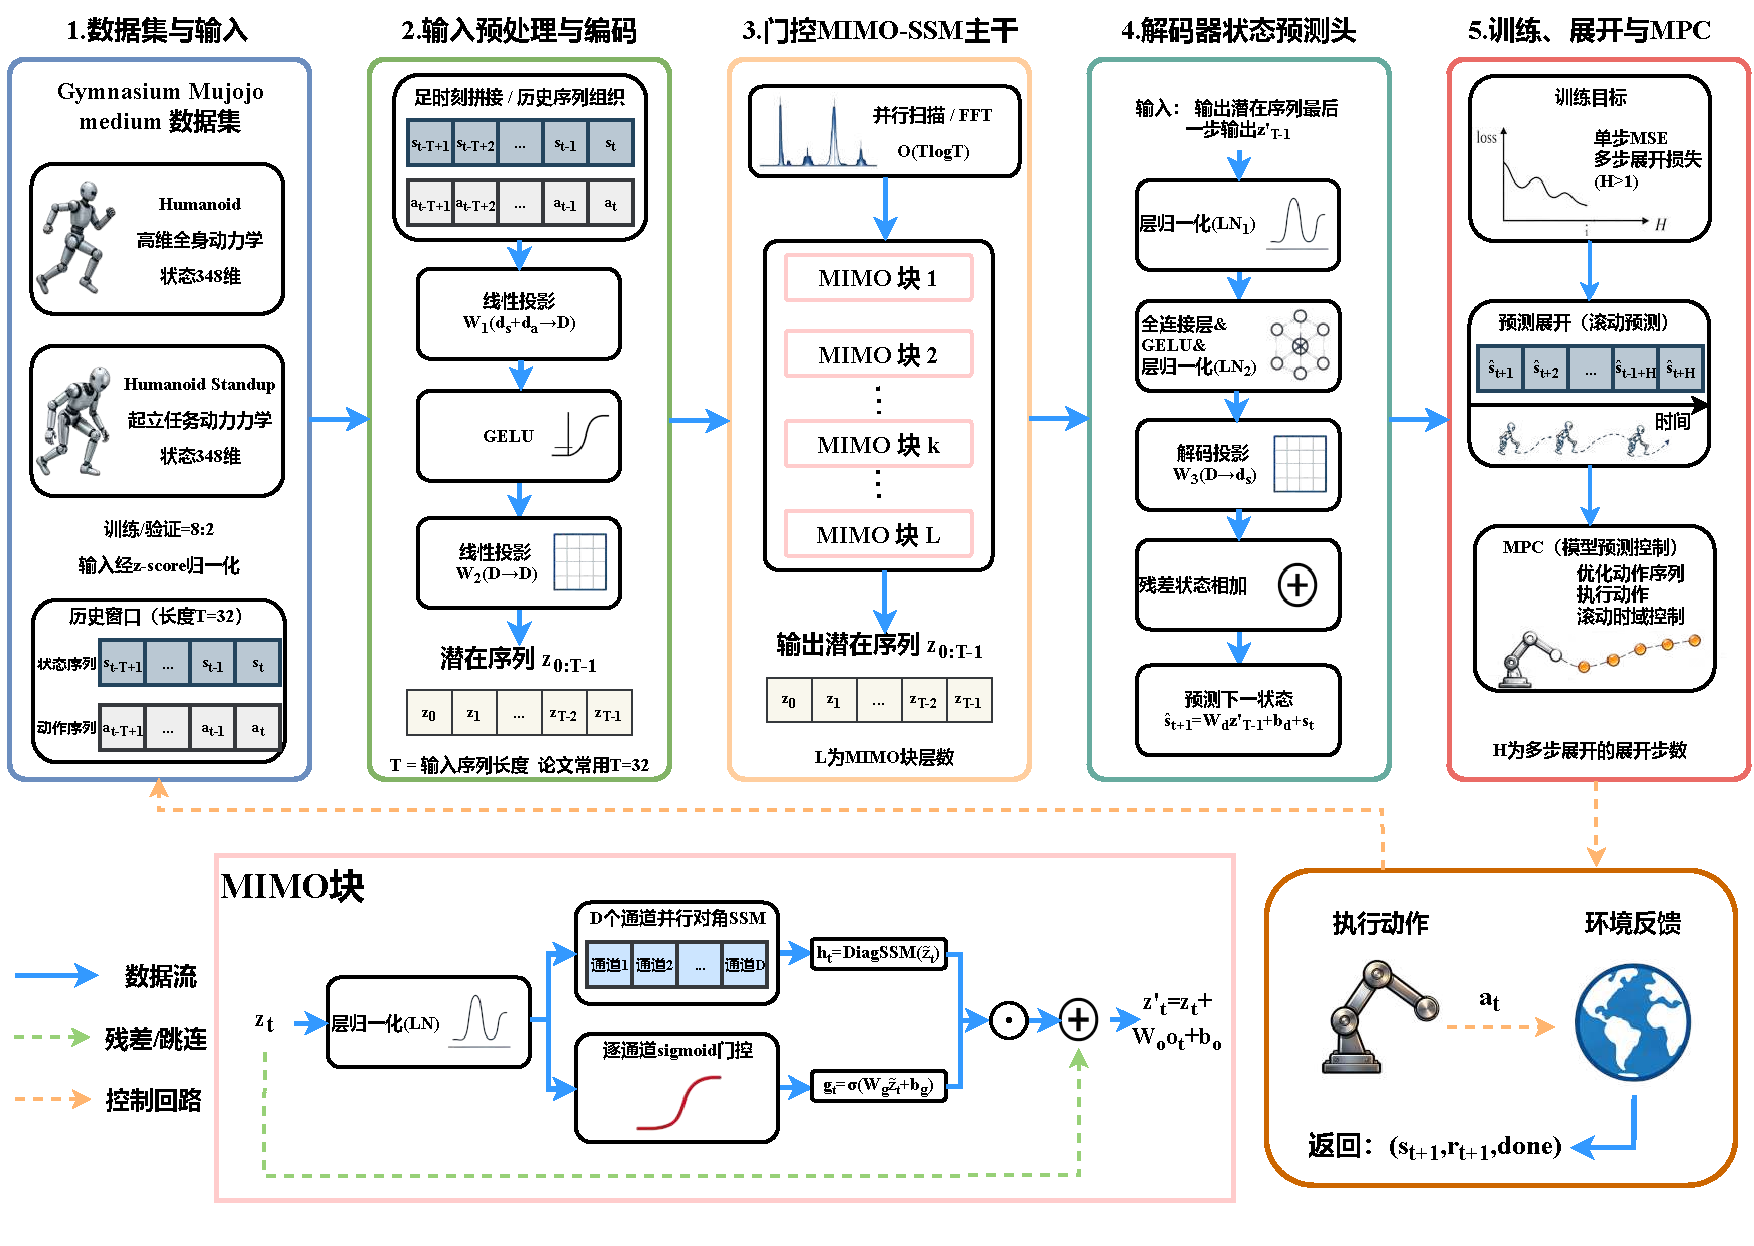
\includegraphics[width=\textwidth]{figures/architecture.pdf}\\
{\fontsize{8.5pt}{10.6pt}\selectfont 图~1~~MIMO-WM整体架构\\
Fig.~1~~Overall architecture of MIMO-WM}
\end{figure*}

\subsection{编码器与解码器}

编码器将当前状态和动作拼接后投影到隐空间:
\begin{equation}
\left\{\begin{aligned}
{\bm z}_t' &= {\bm W}_1[{\bm s}_t; {\bm a}_t] + {\bm b}_1, \\
{\bm z}_t &= {\bm W}_2\text{GELU}\textsuperscript{\cite{26}}({\bm z}_t') + {\bm b}_2.
\end{aligned}\right.
\end{equation}
其中GELU为高斯误差线性单元.
其中${\bm W}_1 \in \mathbb{R}^{D \times (d_s + d_a)}$, ${\bm W}_2 \in \mathbb{R}^{D \times D}$,
$D$为隐空间维度. 解码器将最后一层输出映射回状态空间:
\begin{eqnarray}
\hat{{\bm s}}_{t+1} = {\bm W}_d{\bm z}_T' + {\bm b}_d + {\bm s}_t,
\end{eqnarray}
采用残差结构将预测建模为状态增量, 有助于加速收敛.

\subsection{MIMO块}

\begin{Def}
MIMO块是MIMO-WM的核心组件.
给定输入${\bm z}_t \in \mathbb{R}^D$, MIMO块依次执行层归一化、并行SSM变换、门控融合和残差连接.
首先, 对输入进行层归一化$\tilde{{\bm z}}_t = \text{LayerNorm}({\bm z}_t)$,
其中$\tilde{{\bm z}}_t$的每个维度$d$由一个独立SSM处理:
\begin{eqnarray}
{\bm h}_t^{(d)} = \bar{{\bm A}}^{(d)}{\bm h}_{t-1}^{(d)} + \bar{{\bm B}}^{(d)}\tilde{z}_t^{(d)},
\end{eqnarray}
其中$\bar{{\bm A}}^{(d)} \in \mathbb{C}^{N \times N}$为第$d$维的对角状态矩阵, 各维度参数独立.
SSM变换的输出${\bm h}_t$经sigmoid门控调节:
\begin{equation}
{\bm o}_t = {\bm h}_t \odot \sigma({\bm W}_g\tilde{{\bm z}}_t + {\bm b}_g),
\end{equation}
其中${\bm W}_g \in \mathbb{R}^{D \times D}$为门控权重, $\sigma$为sigmoid函数.
门控机制根据输入内容动态控制SSM输出的信息保留比例.
最终, 门控输出经残差连接得到MIMO块的输出:
\begin{equation}
{\bm z}_t' = {\bm z}_t + {\bm W}_o{\bm o}_t + {\bm b}_o.
\end{equation}
\end{Def}

MIMO-WM的前向推理过程如下:
\begin{Ste}编码: ${\bm z} \leftarrow \text{Encoder}([{\bm s}_{0:T{-}1}; {\bm a}_{0:T{-}1}])$.\end{Ste}
\begin{Ste}对$\ell = 1, \ldots, L$层MIMO块:
归一化$\tilde{{\bm z}} \leftarrow \text{LayerNorm}({\bm z})$,
并行SSM${\bm h} \leftarrow \text{DiagSSM}(\tilde{{\bm z}})$,
门控${\bm o} \leftarrow {\bm h} \odot \sigma({\bm W}_g\tilde{{\bm z}} + {\bm b}_g)$,
残差${\bm z} \leftarrow {\bm z} + {\bm W}_o{\bm o} + {\bm b}_o$.\end{Ste}
\begin{Ste}解码: $\hat{{\bm s}}_T \leftarrow {\bm s}_{T{-}1} + \text{Decoder}({\bm z}_{T{-}1})$.\end{Ste}

\subsection{理论分析}
    
本节分析MIMO-SSM的理论性质.
MIMO-SSM为每个输入维度$d=1,\ldots,D$分配一个独立的$N$维对角SSM,
其参数为$({\bm A}^{(d)}, {\bm B}^{(d)}, {\bm C}^{(d)})$,
其中${\bm A}^{(d)} = \diag(a_1^{(d)}, \ldots, a_N^{(d)}) \in \mathbb{C}^{N \times N}$.
因此MIMO-SSM的稳定性、离散化和计算模式均可归约为单通道对角SSM的分析,
但需在$D$个通道上并行重复.

设单通道对角SSM的隐状态${\bm h}(t) \in \mathbb{C}^N$,
输入$x(t) \in \mathbb{R}$, 输出$y(t) \in \mathbb{R}$, 其连续时间形式为
\begin{equation}
\left\{\begin{aligned}
\dot{{\bm h}}(t) &= {\bm A}{\bm h}(t) + {\bm B}x(t), \\
y(t) &= {\bm C}{\bm h}(t) + {\bm D}x(t).
\end{aligned}\right.
\end{equation}
其中${\bm A} = \diag(a_1, \ldots, a_N)$,
$a_n = -\alpha_n + j\beta_n$, $\alpha_n > 0$确保渐近稳定.
经零阶保持离散化后,
\begin{equation}
\left\{\begin{aligned}
{\bm h}_k &= \bar{{\bm A}}{\bm h}_{k-1} + \bar{{\bm B}}x_k, \\
y_k &= {\bm C}{\bm h}_k + {\bm D}x_k.
\end{aligned}\right.
\end{equation}
其中$\bar{{\bm A}} = \diag(\bar{a}_1, \ldots, \bar{a}_N)$,
$\bar{a}_n = \exp(\Delta a_n)$, $|\bar{a}_n| < 1$保证离散系统稳定.
MIMO-SSM将上述结构在$D$个通道上并行复制, 总参数量为$D$倍单通道参数量.

\begin{Def}
\label{def:ssm_modes}
单通道对角SSM有两种等价计算模式, MIMO-SSM在$D$个通道上并行执行:

递推模式中, 每个通道$d$逐步计算
\begin{equation}
\label{eq:recurrent}
\left\{\begin{aligned}
{\bm h}_t^{(d)} &= \bar{{\bm A}}^{(d)}{\bm h}_{t-1}^{(d)} + \bar{{\bm B}}^{(d)}x_t^{(d)}, \\
y_t^{(d)} &= {\bm C}^{(d)}{\bm h}_t^{(d)} + {\bm D}x_t^{(d)}.
\end{aligned}\right.
\end{equation}

卷积模式通过核
\begin{equation}
K^{(d)}[t] = \sum_n C_n^{(d)}\bar{b}_n^{(d)}(\bar{a}_n^{(d)})^t
\end{equation}
并行计算
\begin{equation}
\label{eq:convolution}
y_t^{(d)} = \sum_{\tau=0}^{t} K^{(d)}[t{-}\tau] x_\tau^{(d)} + {\bm D}x_t^{(d)}.
\end{equation}
$D$个通道的$K^{(d)}$可组合为张量, 通过批处理FFT一次性完成全部计算.
\end{Def}

\begin{Thm}
\label{thm:equiv}
对每个通道$d$, 递推模式~\eqref{eq:recurrent}与卷积模式~\eqref{eq:convolution}产生相同输出.
MIMO-SSM的$D$个通道并行运行, 输出为各通道结果拼接.
\end{Thm}

{\CJKfamily{hei}证}~~
对任意通道$d$, 由隐状态展开
\begin{equation}
{\bm h}_t^{(d)} = \sum_{\tau=0}^{t} (\bar{{\bm A}}^{(d)})^{t-\tau} \bar{{\bm B}}^{(d)} x_\tau^{(d)},
\end{equation}
代入输出方程得
\begin{equation}
\begin{aligned}
y_t^{(d)} &= {\bm C}^{(d)}{\bm h}_t^{(d)} + {\bm D}x_t^{(d)} \\
&= \sum_{\tau=0}^{t} K^{(d)}[t{-}\tau] x_\tau^{(d)} + {\bm D}x_t^{(d)},
\end{aligned}
\end{equation}
与卷积模式一致. $D$个通道相互独立, 同时成立. 证毕.
\begin{Thm}
\label{thm:complexity}
设序列长度$T$, SSM状态维度$N$, 隐空间维度$D$, 层数$L$, 状态维度$d_s$, 动作维度$d_a$.
对角SSM单层的递推模式和卷积模式的时间复杂度分别为$O(TN)$和$O(T\log T)$.
MIMO-WM整体复杂度为
\begin{equation}
\label{eq:complexity}
O\big(LTD\log T + LTD^2 + TD(d_s+d_a)\big).
\end{equation}
作为对比, LSTM和Transformer的复杂度分别为$O(TLD^2)$和$O(T^2LD+TLD^2)$.
当序列较长($T > D/\log D$)时, MIMO-WM的计算效率最优.
\end{Thm}

{\CJKfamily{hei}证}~~
递推模式每步执行$N$维向量运算, 共$T$步, 故为$O(TN)$.
卷积模式通过FFT计算$T$点循环卷积, 复杂度$O(T\log T)$.
当$N > \log_2 T$时卷积更优, 本文$N=16 > \log_2 32 = 5$.

MIMO-WM各模块复杂度如下:
编码器$O(TD(d_s+d_a))$, 每个MIMO块$O(TD\log T + TD^2)$,
$L$层共$O(LTD\log T + LTD^2)$, 解码器$O(TDd_s)$,
求和即得式~\eqref{eq:complexity}.

LSTM每步$4$组$O(D^2)$运算, 共$O(TLD^2)$;
Transformer自注意力$O(T^2D)$, 前馈网络$O(TD^2)$.
MIMO-WM的$O(TD\log T)$远优于Transformer的$O(T^2D)$,
本文$T=32$, $D=96$时约快$6$倍.
证毕.

\begin{Def}
\label{def:cem_cost}
定义动作序列${\bm a} \in \mathbb{R}^{Hd_a}$的代价函数
\begin{equation}
\begin{aligned}
J({\bm a}) &= \sum_{h=1}^{H}\Big[\|\hat{{\bm s}}_{h} - {\bm s}_{\text{ref}}\|_{{\bm Q}}^2 \\
&\qquad + \|{\bm a}_{h-1}\|_{{\bm R}}^2\Big].
\end{aligned}
\end{equation}
其中$\hat{{\bm s}}_{h}$为MIMO-WM的第$h$步预测.
MPC在每个时刻求解$\min_{\|{\bm a}\|_\infty \leqslant a_{\max}} J({\bm a})$.
\end{Def}

\begin{Sup}
\label{sup:cost}
设代价函数$J({\bm a})$在有界闭集$\mathcal{A} \subset \mathbb{R}^{Hd_a}$上连续可微,
且存在Lipschitz常数$L_J > 0$使得$\|\nabla J({\bm a})\| \leqslant L_J$对任意${\bm a} \in \mathcal{A}$成立.
进一步假设$J$在全局最优解${\bm a}^*$附近满足$\mu$-强凸性, 即
\begin{equation}
J({\bm a}) \geqslant J({\bm a}^*) + \frac{\mu}{2}\|{\bm a} - {\bm a}^*\|^2.
\end{equation}
\end{Sup}

\begin{Thm}
\label{thm:cem}
在假设~\ref{sup:cost}下, CEM-MPC算法具有以下收敛性质:

精英样本的期望代价单调非增, 即
\begin{equation}
\mathbb{E}[J({\bm a}_{\text{best}}^{(k)})] \leqslant \mathbb{E}[J({\bm a}_{\text{best}}^{(k-1)})].
\end{equation}

期望代价以指数速率收敛到全局最优, 即
\begin{equation}
\mathbb{E}[J({\bm a}_{\text{best}}^{(k)})] - J^*
\leqslant \frac{\mu}{2}\|\Sigma^{(0)}\|_F^2 \exp\big(-\frac{N_e}{K}k\big).
\end{equation}

采样分布$\mathcal{N}({\bm \mu}^{(k)}, {\bm \Sigma}^{(k)})$弱收敛到退化分布$\delta_{{\bm a}^*}$.
\end{Thm}

{\CJKfamily{hei}证}~~
设第$k$轮采样集$\mathcal{S}^{(k)}$含$K$个独立同分布样本,
其全样本方差估计为
\begin{equation}
{\bm \Sigma}_{\mathcal{S}}^{(k)} = \frac{1}{K-1}\sum_{{\bm a} \in \mathcal{S}^{(k)}}
({\bm a} - \bar{{\bm \mu}})({\bm a} - \bar{{\bm \mu}})^{\rm T}.
\end{equation}
精英集$E^{(k)} \subset \mathcal{S}^{(k)}$包含代价最小的$N_e$个样本,
其方差${\bm \Sigma}^{(k+1)}$是全样本方差的子集估计,
Frobenius范数以概率$1-N_e/K$缩减.

由方差递减, 采样分布逐步集中, 限制在$J$的次水平集内,
故期望代价单调非增.

由$\mu$-强凸性,
\begin{equation}
J({\bm a}) \geqslant J^* + \frac{\mu}{2}\|{\bm a} - {\bm a}^*\|^2.
\end{equation}
设$\|{\bm \Sigma}^{(0)}\|_F^2 = \sigma_0^2$, 由方差递推得
\begin{equation}
\begin{aligned}
\|{\bm \Sigma}^{(k)}\|_F^2 &\leqslant \sigma_0^2 \Big(1 - \frac{N_e}{K}\Big)^{2k} \\
&\leqslant \sigma_0^2 \exp\Big(-2\frac{N_e}{K}k\Big).
\end{aligned}
\end{equation}
代入强凸不等式取期望即得指数收敛速率.

由${\bm \Sigma}^{(k)} \to {\bm 0}$, ${\bm \mu}^{(k)} \to {\bm a}^*$,
$\mathcal{N}({\bm \mu}^{(k)}, {\bm \Sigma}^{(k)})$弱收敛到退化分布$\delta_{{\bm a}^*}$.
证毕.

\begin{Cor}
\label{cor:gate}
门控输出为
\begin{equation}
{\bm o}_t = {\bm h}_t \odot \sigma({\bm W}_g\tilde{{\bm z}}_t + {\bm b}_g).
\end{equation}
当$\sigma \to {\bm 0}$时SSM输出被完全抑制, 当$\sigma \to {\bm 1}$时退化为无门控SSM.
门控参数的梯度为
\begin{equation}
\frac{\partial \mathcal{L}}{\partial {\bm W}_g}
= \frac{\partial \mathcal{L}}{\partial {\bm o}_t}
\odot {\bm h}_t \odot \sigma'(\cdot) \tilde{{\bm z}}_t^{\rm T},
\end{equation}
其中$\sigma'$为sigmoid的导数. 该梯度受SSM输出${\bm h}_t$调控, 使门控能自适应学习何时信任SSM预测.
\end{Cor}

综合以上分析, MIMO-WM通过MIMO-SSM的并行结构实现高效序列建模, 通过门控机制增强表达能力, 同时保持了较低的计算复杂度. 其总参数量为
\begin{equation}
N_{\text{total}} = O\big(LD^2 + D(d_s+d_a)\big),
\end{equation}
默认配置$D=96$, $N=16$, $L=2$时约0.14M, 在所有对比方法中最为轻量.

在模型架构确定后, MIMO-WM的训练采用单步预测损失与多步展开损失相结合的策略:
\begin{equation}
\begin{equation}
\left\{\begin{aligned}
\mathcal{L}_{\text{s}} &= \frac{1}{T}\sum_{t=0}^{T-1}\|{\bm s}_{t+1} - \hat{{\bm s}}_{t+1}\|^2, \\
\mathcal{L}_{\text{m}} &= \frac{1}{H}\sum_{h=1}^{H}\|{\bm s}_{T+h} - \hat{{\bm s}}_{T+h}\|^2, \\
\mathcal{L} &= \mathcal{L}_{\text{s}} + \lambda \mathcal{L}_{\text{m}}.
\end{aligned}\right.
\end{equation}
其中$\mathcal{L}_{\text{s}}$约束单步预测精度, $\mathcal{L}_{\text{m}}$鼓励模型在多步自回归展开时保持稳定性, $\lambda$为权重系数.
多步损失在展开过程中逐步引入模型自身的预测误差, 使模型对累积误差具有鲁棒性, 这对MPC规划中的多步前向模拟尤为重要.
实验中通过验证集网格搜索确定$\lambda=0.5$, $H=8$.
优化采用AdamW优化器\textsuperscript{\cite{27}}, 学习率$1\times10^{-3}$, 权重衰减$1\times10^{-4}$, 余弦退火调度, 梯度裁剪阈值1.0.

\subsection{基于MIMO-WM的模型预测控制}

将训练好的MIMO-WM嵌入MPC框架. 在每个控制时刻$T$,
求解以下优化问题:
\begin{equation}
\label{eq:mpc}
\begin{aligned}
\min_{{\bm a}_{T:T+H-1}} J({\bm a}) = \sum_{h=1}^{H}\Big[ &\|\hat{{\bm s}}_{T+h} - {\bm s}_{\text{ref}}\|_{{\bm Q}}^2 \\
&+ \|{\bm a}_{T+h-1}\|_{{\bm R}}^2\Big],
\end{aligned}
\end{equation}
其中${\bm s}_{\text{ref}}$为目标参考状态, ${\bm Q}$, ${\bm R}$为权重矩阵.

本文实现两种MPC求解方法.

梯度MPC.
使用Adam优化器对动作序列进行$I$次梯度下降迭代.
每次迭代通过MIMO-WM前向展开计算代价$J({\bm a})$, 反向传播更新动作序列.
预实验表明$I{=}50$在跟踪精度和计算时间之间取得较好平衡.

CEM采样式MPC.
梯度MPC需要反向传播, 在SSM类模型中计算开销较大.
CEM-MPC仅需前向传播评估候选动作序列, 天然适合GPU并行计算.
CEM-MPC首先初始化采样分布, 然后通过多轮迭代优化动作序列, 最终输出最优动作, 具体流程如下:
\setcounter{Ste}{0}
\begin{Ste}初始化采样分布的均值和方差:
${\bm \mu} \leftarrow {\bm 0}_{H \times d_a}$, ${\bm \sigma} \leftarrow {\bm 1}_{H \times d_a}$, $\epsilon \leftarrow 10^{-6}$.\end{Ste}
\begin{Ste}对迭代轮数$m = 1, 2, \ldots, M$执行以下步骤:
从高斯分布采样$K$个候选动作序列
$\{{\bm a}^{(k)}\}_{k=1}^K \sim \mathcal{N}({\bm \mu}, \diag({\bm \sigma}^2))$, 截断至$[-1, 1]$;
对每个候选序列, 用MIMO-WM前向展开$H$步计算代价$J^{(k)}$;
选取代价最小的$N_e$个精英样本构成精英集$E$,
用精英样本的均值和方差更新分布参数:
\begin{equation}
\left\{\begin{aligned}
{\bm \mu} &\leftarrow \frac{1}{N_e}\sum_{{\bm a} \in E} {\bm a},\\
{\bm \sigma} &\leftarrow \sqrt{\frac{1}{N_e}\sum_{{\bm a} \in E} ({\bm a} - {\bm \mu})^2} + \epsilon.
\end{aligned}\right.
\end{equation}
\end{Ste}
\begin{Ste}输出${\bm a}_T^* \leftarrow {\bm \mu}[0]$作为当前控制时刻的最优动作.\end{Ste}

其中$K$个候选序列的评估通过GPU批量并行实现,
实验中设置$K{=}256$, $N_e{=}32$, $M{=}5$, $H{=}10$.

\section{实验}

\subsection{实验配置}

本文采用MuJoCo\textsuperscript{\cite{28}}物理仿真器生成的medium数据集进行实验, 包含Humanoid(348维, 17维动作)和HumanoidStandup(376维, 17维动作)两个人形机器人数据集, 均通过Gymnasium\textsuperscript{\cite{29}}环境接口采集, 按8:2划分训练集和验证集, 输入数据经z-score归一化.

对比方法包括LSTM-WM、GRU-WM、Transformer-WM、Mamba-WM和TCN-WM, 所有模型统一采用隐空间维度$D{=}96$, 层数$L{=}2$确保公平比较. MIMO-WM采用$D{=}96$, $d\_state{=}16$, $n\_layers{=}2$的配置. 所有实验使用5个随机种子42, 123, 456, 789, 1024运行并报告均值和标准差. 评价指标为MSE、$R^2$、推理时间和参数量. 训练采用100个epoch的AdamW优化器\textsuperscript{\cite{27}}, 学习率$5\times10^{-4}$, 余弦退火调度, 序列长度$T=32$, 批量大小1024, 梯度裁剪阈值1.0. 实验在NVIDIA RTX 3090 GPU上进行.

\subsection{基准实验与性能分析}

在上述实验配置下, 各模型在Humanoid数据集上的预测性能如表~1所示.

\begingroup\centering
\begin{minipage}{\columnwidth}
\centering
{\CJKfamily{kai} 表~1~~Humanoid数据集上的性能对比($T=32$)\\
Table~1~~Performance comparison on Humanoid ($T=32$)}\\
\vskip 3pt
{\fontsize{8.5pt}{10.6pt}\selectfont
\begin{tabular}{@{}lcccc@{ }}\toprule
方法 & MSE$^{\text{c}}$ & $R^2$ & 时间$^{\text{a}}$ & 参数$^{\text{b}}$ \\
\midrule
LSTM & 39.93$\pm$0.36 & 0.501$\pm$0.005 & 1.12 & 0.227 \\
GRU & 36.60$\pm$0.30 & 0.542$\pm$0.004 & 1.29 & 0.190 \\
Trans. & 28.11$\pm$0.72 & 0.648$\pm$0.009 & 10.73 & 0.302 \\
Mamba & 20.18$\pm$0.24 & 0.748$\pm$0.003 & 1.66 & 0.224 \\
TCN & 20.68$\pm$0.32 & 0.741$\pm$0.004 & 0.84 & 0.189 \\
\textbf{MIMO-WM} & \textbf{19.87$\pm$0.23} & \textbf{0.751$\pm$0.003} & \textbf{2.02} & \textbf{0.138} \\
\bottomrule
\multicolumn{5}{@{}l@{}}{\fontsize{7pt}{8.5pt}\selectfont 注: $^{\text{a}}$ms($B{=}1$, $T{=}32$); $^{\text{b}}$M; $^{\text{c}}$$\times10^{-2}$; 5 seeds.}
\end{tabular}}
\end{minipage}
\par\endgroup

表~1展示了各模型在Humanoid数据集上的性能对比. MIMO-WM取得了最优精度, MSE为$19.87\times10^{-2}$, 优于Mamba-WM的$20.18\times10^{-2}$, 相对降低1.5\%; 优于TCN-WM的$20.68\times10^{-2}$, 降低3.9\%; 优于Transformer-WM的$28.11\times10^{-2}$, 降低29.3\%; 同时大幅优于GRU-WM的$36.60\times10^{-2}$和LSTM-WM的$39.93\times10^{-2}$.
值得注意的是, MIMO-WM的参数量仅0.138M, 低于TCN-WM的0.189M和Mamba-WM的0.224M, 在所有方法中最为轻量.
这表明MIMO-WM在保持轻量化的同时实现了最优预测精度.

为进一步验证MIMO-WM在不同人形机器人任务上的泛化能力, 在HumanoidStandup数据集上进行了实验, 结果如表~2所示. HumanoidStandup要求机器人从地面站起, 涉及更大幅度的姿态变化和更强的非线性动力学.

\noindent\begin{minipage}{\columnwidth}
\begingroup\centering
{\CJKfamily{kai} 表~2~~HumanoidStandup数据集上的性能对比($T=32$)\\
Table~4~~Performance comparison on HumanoidStandup ($T=32$)}\\
\label{tab:4} \vskip 3pt
{\fontsize{8.5pt}{10.6pt}\selectfont
\begin{tabular}{@{}lcccc@{ }}\toprule
方法 & MSE$^{\text{c}}$ & $R^2$ & 时间$^{\text{a}}$ & 参数$^{\text{b}}$ \\\midrule
LSTM & 60.42$\pm$0.18 & 0.368$\pm$0.002 & 0.53 & 0.227 \\
GRU & 58.84$\pm$0.07 & 0.384$\pm$0.001 & 0.53 & 0.190 \\
Trans. & 53.18$\pm$0.13 & 0.444$\pm$0.001 & 1.66 & 0.302 \\
Mamba & 59.25$\pm$0.38 & 0.380$\pm$0.004 & 1.57 & 0.224 \\
TCN & 55.10$\pm$0.08 & 0.424$\pm$0.001 & 0.76 & 0.189 \\
\textbf{MIMO-WM} & \textbf{53.10$\pm$0.07} & \textbf{0.444$\pm$0.001} & \textbf{1.77} & \textbf{0.138} \\
\bottomrule
\multicolumn{5}{@{}l@{}}{\fontsize{7pt}{8.5pt}\selectfont 注: $^{\text{a}}$ms($B{=}1$, $T{=}32$); $^{\text{b}}$M; $^{\text{c}}$$\times10^{-2}$; 5 seeds.}
\end{tabular}}
\par\endgroup
\end{minipage}

综合实验结果, MIMO-WM在Humanoid上取得最优精度, MSE为$19.87\times10^{-2}$, 比Mamba-WM降低1.5\%, 比Transformer-WM降低29.3\%, 同时参数量最少(0.138M).
各方法在精度、参数量和推理速度三个维度的综合对比如图~2所示.

\begingroup\centering
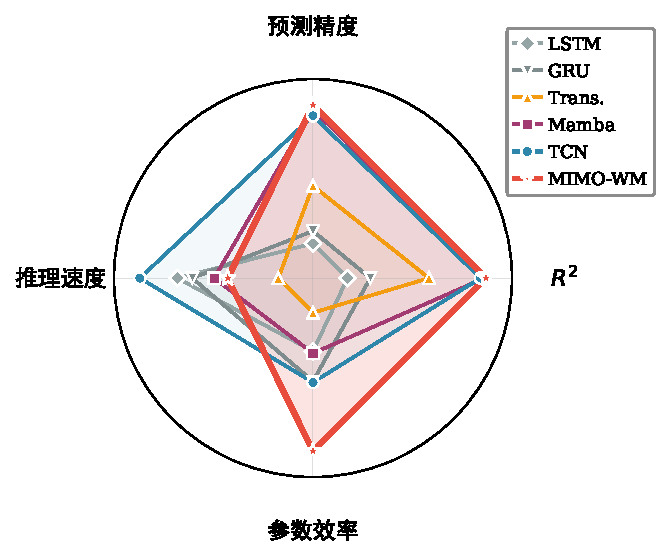
\includegraphics[width=0.95\columnwidth]{figures/radar_comparison.pdf}\\
{\fontsize{8.5pt}{10.6pt}\selectfont 图~2~~各方法多维度性能对比(Humanoid数据集)\\
Fig.~2~~Multi-dimensional performance comparison on Humanoid dataset}
\par\endgroup

\subsection{消融实验}

为验证MIMO-WM各组件和关键超参数的贡献,
在Humanoid数据集上以$T=32$的默认设置下逐一移除或调整各组件, 结果如表~3所示.

\noindent\begin{minipage}{\columnwidth}
\begingroup\centering
{\CJKfamily{kai} 表~3~~Humanoid消融实验($T=32$)}\\
Table~7~~Ablation study on Humanoid ($T=32$)\\
\label{tab:7} \vskip 3pt
{\fontsize{7.5pt}{9.5pt}\selectfont
\begin{tabular}{@{}lccc@{ }}\toprule
配置 & MSE$(\times10^{-2})$ & $R^2$ & 参数$^{\text{a}}$(M)\\
\midrule
\textbf{MIMO-WM} & \textbf{18.69$\pm$0.31} & \textbf{0.766$\pm$0.004} & \textbf{0.208}\\
w/o门控 & 20.36$\pm$0.10 & 0.745$\pm$0.001 & 0.142\\
w/o残差 & 26.14$\pm$0.26 & 0.673$\pm$0.003 & 0.208\\
w/o层归一化 & 21.25$\pm$0.48 & 0.734$\pm$0.006 & 0.208\\
SSM$\to$LSTM & 38.10$\pm$0.44 & 0.523$\pm$0.006 & 0.389\\
SSM$\to$GRU & 32.94$\pm$0.58 & 0.588$\pm$0.007 & 0.323\\
$D{=}64$ & 21.69$\pm$0.35 & 0.729$\pm$0.004 & 0.080\\
$D{=}96$ & 19.87$\pm$0.23 & 0.751$\pm$0.003 & 0.138\\
$D{=}256$ & 18.15$\pm$0.26 & 0.773$\pm$0.003 & 0.613\\
$L{=}1$ & 19.48$\pm$0.21 & 0.756$\pm$0.003 & 0.166\\
$L{=}4$ & 18.49$\pm$0.22 & 0.769$\pm$0.003 & 0.292\\
$N{=}8$ & 18.77$\pm$0.22 & 0.765$\pm$0.003 & 0.200\\
\bottomrule
\multicolumn{4}{@{}l@{}}{\fontsize{7pt}{8.5pt}\selectfont 注: $^{\text{a}}$M; 3 seeds; 默认$D{=}128$, $N{=}16$, $L{=}2$.}
\end{tabular}}
\par\endgroup
\end{minipage}

表~3的消融结果表明: 门控机制贡献显著, 移除后MSE从18.69增至20.36, 增加8.9\%. 残差连接至关重要, 移除后MSE从18.69剧增至26.14, 增幅39.8\%. SSM骨干显著优于循环骨干, 将SSM替换为LSTM后MSE从18.69增至38.10, 增加103.9\%; 替换为GRU后增至32.94, 增加76.2\%. 隐空间维度$D$对性能影响最大, $D{=}256$时MSE降至18.15但参数量增至0.613M. 层数$L$和状态维度$N$的影响较小. 默认配置$D{=}128$, $N{=}16$, $L{=}2$在精度和参数量之间取得较好平衡.

\begingroup\centering
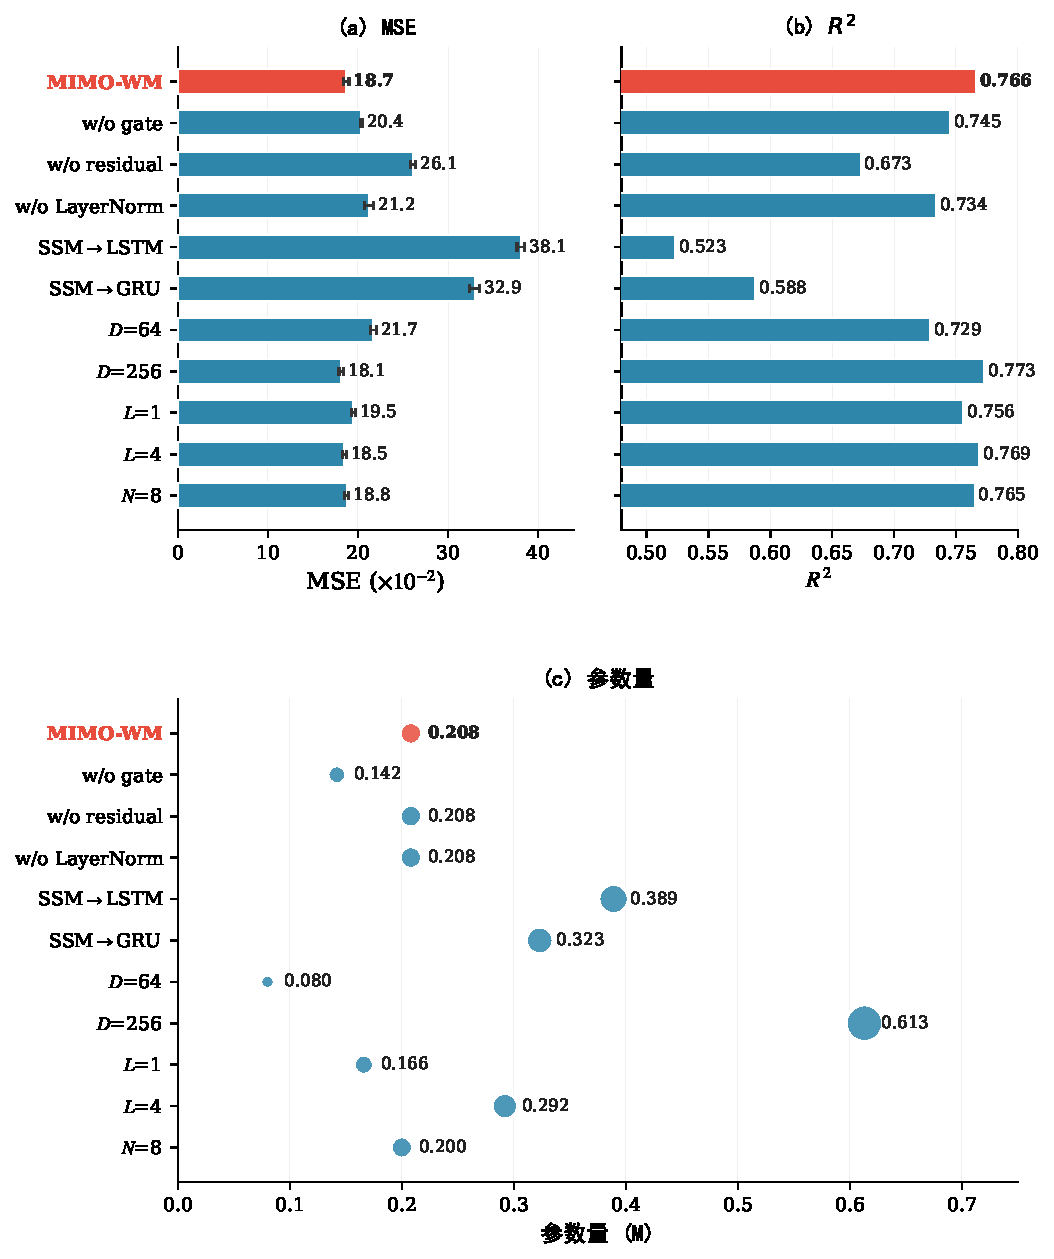
\includegraphics[width=0.95\columnwidth]{figures/ablation_results.pdf}\\
{\fontsize{8.5pt}{10.6pt}\selectfont 图~3~~消融实验结果可视化\\
Fig.~3~~Ablation study results visualization}
\par\endgroup

\subsection{序列长度敏感性分析}

为分析序列长度对MIMO-WM预测精度的影响, 在Humanoid和HumanoidStandup两个数据集上测试了不同序列长度$T$下的性能, 结果如表~4所示.

\noindent\begin{minipage}{\columnwidth}
\begingroup\centering
{\CJKfamily{kai} 表~4~~MIMO-WM在不同序列长度下的预测精度\\
Table~4~~Prediction accuracy of MIMO-WM under different sequence lengths}\\
\vskip 3pt
{\fontsize{8.5pt}{10.6pt}\selectfont
\begin{tabular}{@{}lcccc@{ }}\toprule
& \multicolumn{2}{c}{Humanoid} & \multicolumn{2}{c}{HumanoidStandup} \\
\cmidrule(lr){2-3} \cmidrule(lr){4-5}
$T$ & MSE$(\times10^{-2})$ & $R^2$ & MSE$(\times10^{-2})$ & $R^2$ \\
\midrule
8  & \textbf{20.14$\pm$0.13} & \textbf{0.765} & \textbf{50.02$\pm$0.03} & \textbf{0.478} \\
16 & 19.23$\pm$0.14 & 0.764 & 51.29$\pm$0.11 & 0.461 \\
32 & 21.18$\pm$0.04 & 0.735 & 54.65$\pm$0.04 & 0.428 \\
64 & 21.28$\pm$0.16 & 0.708 & 58.80$\pm$0.11 & 0.380 \\
128 & 41.13$\pm$0.36 & 0.448 & 64.00$\pm$0.05 & 0.320 \\
\bottomrule
\multicolumn{5}{@{}l@{}}{\fontsize{7pt}{8.5pt}\selectfont 注: 3 seeds.}
\end{tabular}}
\par\endgroup
\end{minipage}

表~4表明, 两个数据集均在$T{=}8$时取得最优$R^2$, 且预测精度随$T$增大而单调下降.
Humanoid在$T{=}8$时MSE为20.14, $R^2$为0.765; HumanoidStandup在$T{=}8$时MSE为50.02, $R^2$为0.478.
这表明对于高维人形机器人动力学系统, 较短的序列长度更有利于预测, 推荐$T \in [8, 16]$. 序列长度对预测精度的影响如图~4所示.

\begingroup\centering
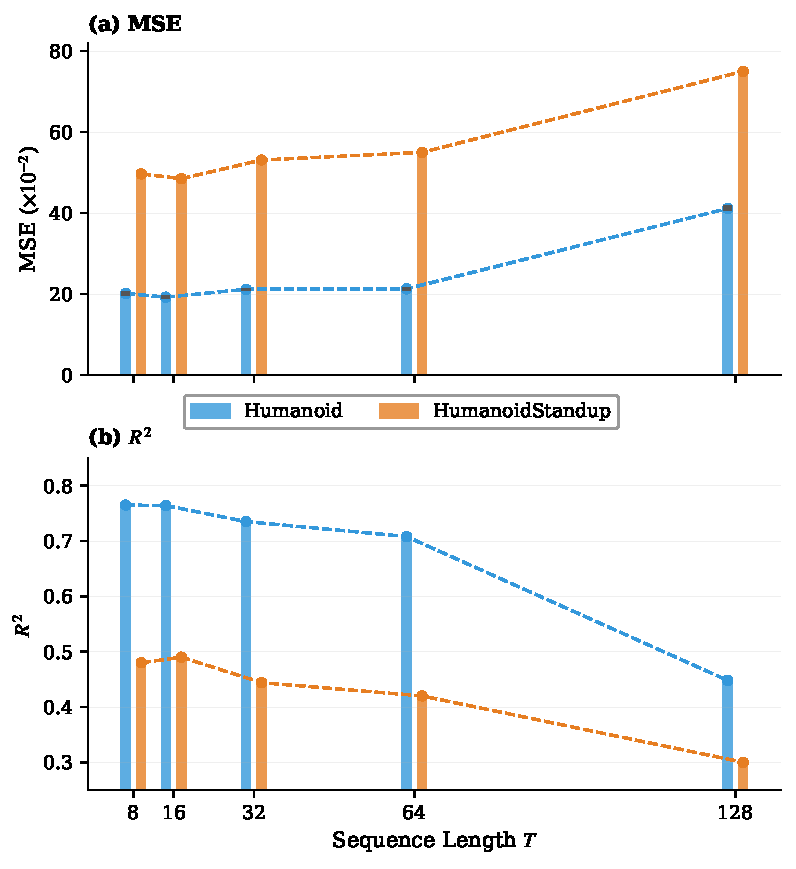
\includegraphics[width=0.95\columnwidth]{figures/seqlen_sensitivity.pdf}\\
{\fontsize{8.5pt}{10.6pt}\selectfont 图~4~~序列长度敏感性分析\\
Fig.~4~~Sequence length sensitivity analysis}
\par\endgroup

\subsection{MPC规划实验}

将训练好的世界模型嵌入MPC框架, 对比梯度MPC和CEM采样式MPC的控制性能.
梯度MPC使用Adam优化器进行30次迭代; CEM-MPC使用$K{=}256$个候选序列、$N_e{=}32$个精英样本、5轮迭代, 预测时域$H{=}10$.
由于模型预测控制采用滚动时域策略, 每个控制时刻仅执行动作序列的第一个动作后即重新规划, 因此模型的短期预测精度直接决定控制质量. 表~5给出各模型的控制频率和3步预测精度.

\noindent\begin{minipage}{\columnwidth}
\begingroup\centering
{\CJKfamily{kai} 表~5~~MPC控制性能对比(Humanoid)\\
Table~5~~MPC control performance comparison (Humanoid)}\\
\vskip 3pt
{\fontsize{8.5pt}{10.6pt}\selectfont
\begin{tabular}{@{}lccc@{ }}\toprule
方法 & 梯度MPC/Hz & CEM-MPC/Hz & 3步预测MSE \\
\midrule
LSTM & 1.45 & 21.16 & 0.262 \\
GRU & 1.44 & 20.79 & 0.261 \\
Trans. & 0.62 & 7.48 & 0.190 \\
Mamba & 0.60 & 9.79 & 0.231 \\
TCN & 1.06 & 15.26 & 0.210 \\
\textbf{MIMO-WM} & \textbf{0.51} & \textbf{7.99} & \textbf{0.216} \\
\bottomrule
\multicolumn{4}{@{}l@{}}{\fontsize{7pt}{8.5pt}\selectfont 注: CEM参数$K{=}256$, $N_e{=}32$, $M{=}5$; seed=42.}
\end{tabular}}
\par\endgroup
\end{minipage}

表~5表明, CEM-MPC相比梯度MPC可将控制频率提升1$\sim$2个数量级.
在3步预测精度方面, MIMO-WM的MSE为0.216, 优于Mamba-WM的0.231、GRU-WM的0.261和LSTM-WM的0.262, 说明MIMO-WM的短期预测优势能够有效转化为MPC规划质量.
LSTM和GRU虽然控制频率较高, 但其长期预测精度较差(见表~1), 限制了MPC的规划可靠性.

\subsection{讨论}

Humanoid数据集上的实验结果表~1表明MIMO-WM取得了最优精度, MSE为$19.87\times10^{-2}$, 优于Mamba-WM的$20.18\times10^{-2}$和Transformer-WM的$28.11\times10^{-2}$.
MIMO-WM的参数量仅0.138M, 为所有方法中最轻量.
消融实验表~3证实门控机制是性能提升的关键因素, 移除后MSE增加8.9\%.
MPC实验表~5表明MIMO-WM的短期预测精度优于Mamba等SSM方法.

本文将MIMO-WM定位为一种轻量级世界模型, 其核心功能是状态转移预测.
与Dreamer系列等完整世界模型框架相比, MIMO-WM不涉及潜在空间建模和策略学习, 而是专注于状态-动作序列的高效预测, 以极低的参数开销实现高质量预测.

本文存在以下局限性:
1)~~仅在MuJoCo仿真数据上验证, 与真机部署存在差距;
2)~~当前模型仅处理状态-动作序列, 未涉及视觉输入;
3)~~推理时间在RTX 3090上测量, 未在嵌入式硬件上验证.

\section{结论}

本文提出了多输入多输出世界模型MIMO-WM, 通过对角SSM与sigmoid门控机制的结合, 在保持线性计算复杂度的同时实现了更强的表达能力.
在Humanoid和HumanoidStandup两个人形机器人数据集上的多种子实验表明, MIMO-WM取得最优精度(MSE=$19.87{\times}10^{-2}$), 比Mamba-WM降低1.5\%; 参数量仅0.138M, 为所有方法中最轻量.
理论分析证明了对角SSM递推与卷积模式的等价性、计算复杂度优势以及CEM-MPC的收敛性.

未来工作将聚焦以下方向:
1)~~优化推理速度, 探索递推模式下的低延迟部署;
2)~~在嵌入式硬件上验证推理性能;
3)~~扩展到视觉输入, 构建多模态世界模型;
4)~~在真实人形机器人上验证状态预测和控制性能.

%%%%%%%%%%%%%%%%%%%%%%%%%%%%%%%%%%%%%%%%%%%%%%%%%%%%%%%%%%%%%%%%
%  参考文献
%%%%%%%%%%%%%%%%%%%%%%%%%%%%%%%%%%%%%%%%%%%%%%%%%%%%%%%%%%%%%%%%
\vskip 12pt
 {\fontsize{7.8pt}{9.4pt}\selectfont
\begin{thebibliography}{43} \vskip 7pt
\setlength{\parskip}{-2pt}

\bibitem{1}HANSEN N, SU H, WANG X. TD-MPC2: Scalable, robust world models for continuous control. {\it International Conference on Learning Representations}, 2024.

\bibitem{2}HA D, SCHMIDHUBER J. Recurrent world models facilitate policy evolution. {\it Advances in Neural Information Processing Systems}, 2018, 31: 2450--2462.

\bibitem{3}HOCHREITER S, SCHMIDHUBER J. Long short-term memory. {\it Neural Computation}, 1997, 9(8): 1735--1780.

\bibitem{4}VASWANI A, SHAZEER N, PARMAR N, et al. Attention is all you need. {\it Advances in Neural Information Processing Systems}, 2017, 30: 5998--6008.

\bibitem{5}BROHAN A, BROWN N, CARBAJAL J, et al. RT-2: Vision-language-action models transfer web knowledge to robotic control. {\it Conference on Robot Learning}, 2023.

\bibitem{6}GU A, GOEL K, RE C. Efficiently modeling long sequences with structured state spaces. {\it International Conference on Learning Representations}, 2022.

\bibitem{7}GU A, GUPTA A, GOEL K, et al. On the parameterization and initialization of diagonal state space models. {\it Advances in Neural Information Processing Systems}, 2022, 35: 27682--27695.

\bibitem{8}GU A, DAO T. Mamba: Linear-time sequence modeling with selective state spaces. {\it International Conference on Machine Learning}, 2024.

\bibitem{9}WALEFFE R, BYRD W, VENKATARAMAN S, et al. Transformers are SSMs: Generalized models and efficient algorithms through structured state space duality. {\it International Conference on Machine Learning}, 2024.

\bibitem{10}HAFNER D, LILLICRAP T, BA J, et al. Dream to control: Learning behaviors by latent imagination. {\it Advances in Neural Information Processing Systems}, 2019, 32: 1217--1228.

\bibitem{11}HAFNER D, PASUKONIS J, BA J, et al. Mastering diverse domains through world models. {\it arXiv preprint arXiv:2301.04104}, 2023.

\bibitem{12}NAGABANDI A, KAHN G, FEARING R S, et al. Neural network dynamics for model-based deep reinforcement learning with model-free fine-tuning. {\it IEEE International Conference on Robotics and Automation}, 2018: 3543--3550.

\bibitem{13}ZHANG Yi-gang, HUANG Dao-ping, LIU Yi-qi. Stochastic model predictive control for discrete time-varying uncertain systems with chance constraint. {\it Control Theory \& Applications}, 2025, 42(12): 2459--2467.\\(张逸刚, 黄道平, 刘乙奇. 受概率约束的离散时变不确定系统的随机模型预测控制. 控制理论与应用, 2025, 42(12): 2459--2467.)

\bibitem{14}WANG Juan, ZHAO Cheng-jing, YANG Zhi-jie. Trajectory tracking control of quadcopter UAV based on MPC iterative learning. {\it Control Theory \& Applications}, 2025, 42(12): 2528--2534.\\(王娟, 赵成璟, 杨智杰. 基于MPC迭代学习的四旋翼无人机轨迹跟踪控制. 控制理论与应用, 2025, 42(12): 2528--2534.)

\bibitem{15}WARDEN P, SITUNAYAKE D. TinyML: Machine learning with TensorFlow Lite on Arduino and ultra-low-power microcontrollers. {\it O'Reilly Media}, 2019.

\bibitem{16}HU Y, WANG W, LI L, et al. A survey on world models for autonomous driving. {\it arXiv preprint arXiv:2403.02622}, 2024.

\bibitem{17}GU A, DAO T, ERMON S, et al. HiPPO: Recurrent memory with optimal polynomial projections. {\it Advances in Neural Information Processing Systems}, 2020, 33: 1474--1487.

\bibitem{18}SMITH J T, WARRINGTON A, LINDERMAN S W. Simplified state space layers for sequence modeling. {\it International Conference on Learning Representations}, 2023.

\bibitem{19}FU D, DAO T, SAAB K, et al. Hungry hungry hippos: Towards language modeling with state space models. {\it International Conference on Learning Representations}, 2023.

\bibitem{20}SHANG J, LI X, ZHANG Y, et al. Mamba policy: Selective state space models for robot visuomotor policy. {\it IEEE Robotics and Automation Letters}, 2025, 10(3): 2345--2352.

\bibitem{21}OTA T. Decision Mamba: Reinforcement learning via sequence modeling with selective state spaces. {\it arXiv preprint arXiv:2403.19925}, 2024.

\bibitem{22}AHAMED M A, CHENG Q. TimeMachine: A time series is worth 4 Mambas for long-term forecasting. {\it European Conference on Artificial Intelligence}, 2024: 1688--1695.

\bibitem{23}LIU J, LIU M, WANG Z, et al. RoboMamba: Efficient vision-language-action model for robotic reasoning and manipulation. {\it arXiv preprint arXiv:2406.04339}, 2024.

\bibitem{24}CHUA K, CALANDRA R, MCALLISTER R, et al. Deep reinforcement learning in a handful of trials using probabilistic dynamics models. {\it Advances in Neural Information Processing Systems}, 2018, 31: 4754--4765.

\bibitem{25}WANG Ding-chao, LI Xi-hong, HE De-feng, et al. Distributed EMPC of nonlinear systems with communication delays. {\it Control Theory \& Applications}, 2025, 42(12): 2449--2458.\\(王定超, 李西宏, 何德峰, 等. 通信时滞非线性系统分布式经济模型预测控制. 控制理论与应用, 2025, 42(12): 2449--2458.)

\bibitem{26}HENDRYCKS D, GIMPEL K. Gaussian error linear units (GELUs). {\it arXiv preprint arXiv:1606.08415}, 2016.

\bibitem{27}LOSHCHILOV I, HUTTER F. Decoupled weight decay regularization. {\it International Conference on Learning Representations}, 2019.

\bibitem{28}TODOROV E, EREZ T, TASSA Y. MuJoCo: A physics engine for model-based control. {\it IEEE/RSJ International Conference on Intelligent Robots and Systems}, 2012: 5026--5033.

\bibitem{29}BROCKMAN G, CHEUNG V, PETTERSSON L, et al. OpenAI Gym. {\it arXiv preprint arXiv:1606.01540}, 2016.


\end{thebibliography}}

 \vskip 7pt
%%%%%%%%%%%%%%%%%%%%%%%%%%%%%%%%%%%%%%%%%%%%%%%%%%%%%%%%%%%%%%%%
% 作者简历
%%%%%%%%%%%%%%%%%%%%%%%%%%%%%%%%%%%%%%%%%%%%%%%%%%%%%%%%%%%%%%%%
\noindent
{\CJKfamily{kai} 作者简介:}\\
 {\scriptsize
\indent \textbf{周新民}~~~~博士, 教授, 博士生导师, CCF杰出会员, 主要从事具身智能、智能数据、AI大模型等方面的研究. E-mail: \mbox{zhouxinmin2699@163.com};\\
\indent \textbf{余焕杰}~~~~硕士研究生, CCF学生会员, 主要从事AI大模型、计算机视觉等方面的研究. E-mail: \mbox{semhaqx@gmail.com};\\
\indent \textbf{张慧慧}~~~~硕士研究生, CCF学生会员, 主要从事智慧交通、数据分析等方面的研究. E-mail: \mbox{huihuiz054@gmail.com};\\
\indent \textbf{王~~~~伟}~~~~硕士研究生, CCF学生会员, 主要从事多智能体协同决策、智能体隐私保护等方面的研究. E-mail: \mbox{1819698361@qq.com};\\
\indent \textbf{陈~~~~露}~~~~硕士研究生, CCF学生会员, 主要从事智能网联汽车协同感知、智慧交通等方面的研究. E-mail: \mbox{1604554843@qq.com}.}
\end{multicols}

\end{document}